\documentclass[a4paper]{article}
% Этот шаблон документа разработан в 2014 году
% Данилом Фёдоровых (danil@fedorovykh.ru) 
% для использования в курсе 
% <<Документы и презентации в \LaTeX>>, записанном НИУ ВШЭ
% для Coursera.org: http://coursera.org/course/latex .
% Исходная версия шаблона --- 
% https://www.writelatex.com/coursera/latex/5.3

% В этом документе преамбула

\usepackage{siunitx}
%%% Работа с русским языком
%\usepackage{cmap}					% поиск в PDF
%\usepackage{mathtext} 				% русские буквы в формулах
%\usepackage[T2A]{fontenc}			% кодировка
%\usepackage[utf8]{inputenc}			% кодировка исходного текста
%\usepackage[english,russian]{babel}	% локализация и переносы
%\usepackage{indentfirst}
%\frenchspacing
%
%\renewcommand{\epsilon}{\ensuremath{\varepsilon}}
%\newcommand{\phibackup}{\ensuremath{\phi}}
%\renewcommand{\phi}{\ensuremath{\varphi}}
%\renewcommand{\varphi}{\ensuremath{\phibackup}}
%\renewcommand{\kappa}{\ensuremath{\varkappa}}
%\renewcommand{\le}{\ensuremath{\leqslant}}
%\renewcommand{\leq}{\ensuremath{\leqslant}}
%\renewcommand{\ge}{\ensuremath{\geqslant}}
%\renewcommand{\geq}{\ensuremath{\geqslant}}
%\renewcommand{\emptyset}{\varnothing}
%\renewcommand{\Im}{\operatorname{Im}}
%\renewcommand{\Re}{\operatorname{Re}}


%%% Дополнительная работа с математикой
\usepackage{amsmath,amsfonts,amssymb,amsthm,mathtools} % AMS
%\usepackage{icomma} % "Умная" запятая: $0,2$ --- число, $0, 2$ --- перечисление

%% Номера формул
%\mathtoolsset{showonlyrefs=true} % Показывать номера только у тех формул, на которые есть \eqref{} в тексте.
%\usepackage{leqno} % Нумереация формул слева

%% Свои команды
\DeclareMathOperator{\sgn}{\mathop{sgn}}
\DeclareMathOperator{\sign}{\mathop{sign}}
\DeclareMathOperator*{\res}{\mathop{res}}
\DeclareMathOperator*{\tr}{\mathop{tr}}
\DeclareMathOperator*{\rot}{\mathop{rot}}
\DeclareMathOperator*{\divop}{\mathop{div}}
\DeclareMathOperator*{\grad}{\mathop{grad}}

%% Перенос знаков в формулах (по Львовскому)
\newcommand*{\hm}[1]{#1\nobreak\discretionary{}
{\hbox{$\mathsurround=0pt #1$}}{}}

%%% Работа с картинками
\usepackage{graphicx}  % Для вставки рисунков
\graphicspath{{figures/}}  % папки с картинками
\setlength\fboxsep{3pt} % Отступ рамки \fbox{} от рисунка
\setlength\fboxrule{1pt} % Толщина линий рамки \fbox{}
\usepackage{wrapfig} % Обтекание рисунков текстом

%%% Работа с таблицами
\usepackage{array,tabularx,tabulary,booktabs} % Дополнительная работа с таблицами
\usepackage{longtable}  % Длинные таблицы
\usepackage{multirow} % Слияние строк в таблице

%%% Теоремы
\theoremstyle{plain} % Это стиль по умолчанию, его можно не переопределять.
\newtheorem{thm}{Теорема}
\newtheorem*{thm*}{Теорема}
\newtheorem{prop}{Предложение}
\newtheorem*{prop*}{Предложение}
 
\theoremstyle{definition} % "Определение"
%\newtheorem{corollary}{Следствие}[theorem]
\newtheorem{dfn}{Определение}
\newtheorem*{dfn*}{Определение}
\newtheorem{prob}{Задача}
\newtheorem*{prob*}{Задача}

 
\theoremstyle{remark} % "Примечание"
\newtheorem*{sol}{Решение}
\newtheorem*{rem}{Замечание}

%%% Программирование
\usepackage{etoolbox} % логические операторы

%%% Страница
%\usepackage{extsizes} % Возможность сделать 14-й шрифт
%\usepackage{geometry} % Простой способ задавать поля
%	\geometry{top=25mm}
%	\geometry{bottom=35mm}
%	\geometry{left=35mm}
%	\geometry{right=20mm}
 
\usepackage{fancyhdr} % Колонтитулы
%	\pagestyle{fancy}
 %	\renewcommand{\headrulewidth}{0pt}  % Толщина линейки, отчеркивающей верхний колонтитул
	%\lfoot{Нижний левый}
	%\rfoot{Нижний правый}
	%\rhead{Верхний правый}
	%\chead{Верхний в центре}
	%\lhead{Верхний левый}
	%\cfoot{Нижний в центре} % По умолчанию здесь номер страницы

\usepackage{setspace} % Интерлиньяж
%\onehalfspacing % Интерлиньяж 1.5
%\doublespacing % Интерлиньяж 2
%\singlespacing % Интерлиньяж 1

\usepackage{lastpage} % Узнать, сколько всего страниц в документе.

\usepackage{soul} % Модификаторы начертания

\usepackage{hyperref}
\usepackage[usenames,dvipsnames,svgnames,table,rgb]{xcolor}
\hypersetup{				% Гиперссылки
    unicode=true,           % русские буквы в раздела PDF
    pdftitle={Заголовок},   % Заголовок
    pdfauthor={Автор},      % Автор
    pdfsubject={Тема},      % Тема
    pdfcreator={Создатель}, % Создатель
    pdfproducer={Производитель}, % Производитель
    pdfkeywords={keyword1} {key2} {key3}, % Ключевые слова
%    colorlinks=true,       	% false: ссылки в рамках; true: цветные ссылки
    %linkcolor=red,          % внутренние ссылки
    %citecolor=black,        % на библиографию
    %filecolor=magenta,      % на файлы
    %urlcolor=cyan           % на URL
}

\usepackage{csquotes} % Еще инструменты для ссылок

%\usepackage[style=apa,maxcitenames=2,backend=biber,sorting=nty]{biblatex}

\usepackage{multicol} % Несколько колонок

\usepackage{tikz} % Работа с графикой
\usepackage{pgfplots}
\usepackage{pgfplotstable}
%\usepackage{coloremoji}
\usepackage{floatrow}
\usepackage{subcaption}
\graphicspath{{figures/}}

\renewcommand\thesubfigure{\asbuk{subfigure}}
%\addbibresource{master.bib}

\usepackage{import}
\usepackage{pdfpages}
\usepackage{transparent}
\usepackage{xcolor}
\usepackage{xifthen}

\newcommand{\incfig}[2][1]{%
    \def\svgwidth{#1\columnwidth}
    \import{./figures/}{#2.pdf_tex}
}
%\usepackage{titlesec}
%\titleformat{\section}{\normalfont\Large\bfseries}{}{0pt}{}
%----------------------STANDART:
%\titleformat{\chapter}[display]
%  {\normalfont\huge\bfseries}{\chaptertitlename\ \thechapter}{20pt}{\Huge}
%\titleformat{\section}{\normalfont\Large\bfseries}{\thesection}{1em}{}
%\titleformat{\subsection}
%  {\normalfont\large\bfseries}{\thesubsection}{1em}{}
%\titleformat{\subsubsection}
%  {\normalfont\normalsize\bfseries}{\thesubsubsection}{1em}{}
%\titleformat{\paragraph}[runin]
%  {\normalfont\normalsize\bfseries}{\theparagraph}{1em}{}
%\titleformat{\subparagraph}[runin]
%  {\normalfont\normalsize\bfseries}{\thesubparagraph}{1em}{}

\pdfsuppresswarningpagegroup=1
\pgfplotsset{compat=1.16}



%\setcounter{tocdepth}{1} % only parts,chapters,sections
%\titleformat{\subsection}{\normalfont\large\bfseries}{}{0em}{}
%\titleformat{\subsubsection}{\normalfont\normalsize\bfseries}{}{0em}{}

%\newcommand{\textover}[2]{\stackrel{\mathclap{\normalfont\mbox{#2}}}{#1}}

\author{Yaroslav Drachov\\
Moscow Institute of Physics and Technology}
%\author{Драчов Ярослав\\
%Факультет общей и прикладной физики МФТИ}
\newcommand{\veq}{\mathrel{\rotatebox{90}{$=$}}}
%\newcommand{\teto}[1]{\stackrel{\mathclap{\normalfont\tiny\mbox{#1}}}{\to}}
%\renewcommand{\thesubsection}{\arabic{subsection}}

%%\setcounter{secnumdepth}{0}

\definecolor{tabblue}{RGB}{30, 119, 180}
\definecolor{taborange}{RGB}{255, 127, 15}
\definecolor{tabgreen}{RGB}{45, 160, 43}
\definecolor{tabred}{RGB}{214, 38, 40}
\definecolor{tabpurple}{RGB}{148, 103, 189}
\definecolor{tabbrown}{RGB}{140, 86, 76}
\definecolor{tabpink}{RGB}{227, 119, 193}
\definecolor{tabgray}{RGB}{127, 127, 127}
\definecolor{tabolive}{RGB}{188, 189, 33}
\definecolor{tabcyan}{RGB}{22, 190, 207}
\pgfplotscreateplotcyclelist{colorbrewer-tab}{
{tabblue},
{taborange},
{tabgreen},
{tabred},
{tabpurple},
{tabbrown},
{tabpink},
{tabgray},
{tabolive},
{tabcyan},
}
\usepackage{csvsimple}
\usepackage{extarrows}
%\renewcommand{\labelenumii}{\asbuk{enumii})}
%\renewcommand{\labelenumiv}{\Asbuk{enumiv}}
%\newcommand{\prob}[1]{\subsubsection*{#1}}
\sisetup{output-decimal-marker = {,},separate-uncertainty = true,exponent-product = \cdot}

\usepackage{braket}
\usepackage{enumerate}
\usepackage{chngcntr}
%\counterwithin*{equation}{problem}
%\usepackage{bbold}

\newtheoremstyle{hiProb}% ⟨name ⟩ 
{3pt}% ⟨Space above ⟩1 
{3pt}% ⟨Space below ⟩1
{}% ⟨Body font ⟩
{}% ⟨Indent amount ⟩2
{\bfseries}% ⟨Theorem head font⟩
{.}% ⟨Punctuation after theorem head ⟩
{.5em}% ⟨Space after theorem head ⟩3
%{\thmname{#1} \thmnote{#3}}% ⟨Theorem head spec (can be left empty, meaning ‘normal’)⟩
{\thmnote{#3}}% ⟨Theorem head spec (can be left empty, meaning ‘normal’)⟩
\theoremstyle{hiProb} % "Определение"
%\newtheorem{hiProb}{Задача}
\newtheorem{hiProb}{}
%\usepackage{mmacells}
\newcommand{\textover}[2]{\stackrel{\mathclap{\normalfont\scriptsize\mbox{#2}}}{#1}}
\usepackage{units}
\usepackage[math]{cellspace}%
\setlength\cellspacetoplimit{2pt}
\setlength\cellspacebottomlimit{2pt}

\DeclareMathAlphabet{\mathbbold}{U}{bbold}{m}{n}

\newcommand{\normord}[1]{:\mathrel{#1}:}

\title{Домашняя работа по вычислительной математике\\
Задание 1}
\begin{document}
	\maketitle
	\section*{Тема IX. Построение общего решения}	
\begin{hiProb}[7.19]
	Найти все решения задачи на собственные значения
	\[
		\frac{y_{k+1} -2 y_k +y_{k-1}}{h^2}=(2-\lambda)
		y_k,\quad y_0=0,\quad y_N=y_{N-1},\quad
		h=\frac{1}{N}
	.\] 

\end{hiProb}
\begin{sol}
Рассмотрим эту задачу как разностное уравнение второго порядка
\[
	y_{k+1}-2y_k+ y_{k-1}=(2-\lambda)h^2 y_k
\]
или
\[
	y_{k+1}+(\lambda h^2 -4)y_k +y_{k-1}=0
.\] 
Характеристическое уравнение, соответствующее данному разностному,
есть
\[
	q^2 +(\lambda h^2 -4) q+1=0
.\] 
По теореме Виета имеем
\[
q_1= \frac{1}{q_2}
.\] 
Тогда общее решение разностного уравнения имеет вид
\[
\overline{y}_n= \alpha q_1^n +\beta q_1^{-n}
.\] 
Подстановка в левое граничное условие даёт соотношение
$\alpha+\beta=0$, тогда
\[
	\overline{y}= \alpha\left(  q_1^n-q_1^{-n} \right) 
.\] 
Теперь используем правое граничное условие
\[
	\alpha\left( q_1^N-q_1^{-N} \right) =
	\alpha\left( q_{1}^{N-1}-q_1^{-N+1} \right) 
.\] 
При $\alpha=0$ получаем тривиальное решение, которое нас не 
интересует. Тогда для того, чтобы удовлетворить этому уравнению,
должно быть выполнено \[q_1^{N}-q_1^{-N}=q_1^{N-1}-q_1^{1-N}.\]
\[
q_1^{2N}-1=q_1^{2N-1}-q_1
.\] 
\[
	(q_1^{2N-1}+1)(q_1-1)=0
.\] 
Откуда
\[
	q_1=e^{\frac{\pi(1+2k)i}{2N-1}},\
	k=0,\,1,\ldots,\,N-2;\quad
	q_1=1\text{ --- тривиальное решение}
.\] 
Подстановка полученного решения позволяет получить решение
разностного уравнения
\[
	\overline{y}_n ^{(k)}= \alpha \left( 
		\exp \left( \frac{\pi (1+2k) n i}{2N-1} \right) -
	\exp \left( - \frac{\pi (1+2k) n i}{2N-1} \right) \right) =\alpha 2 i \sin \frac{\pi(2k+1)n}{2N-1}
.\] 
Выбирая $\alpha=\frac{1}{2i}\sqrt{\frac{2}{l}} $, получаем
собственные функции
\[
	\overline{y}_n^{(k)}= \frac{2}{l}\sin \frac{\pi(2k+1)n}{2N-1}
.\] 
Подстановка собственных функций позволяет после ряда
тригонометрических преобразований найти спектр
для $k=0,\ldots,\,N-2$:
\begin{multline*}
	\lambda_{(k)}=2 - \frac{y_{m+1}^{(k)}-2 y_{m}^{(k)}+
	y_{m-1}^{(k)}}{y_m^{(k)}h^2}=\\=
	2- \frac{1}{h^2} \left( 
		\frac{\sin \frac{\pi (2k+1)(m+1)}{2N-1}  -
	2 \sin \frac{\pi (2k+1)m}{2N-1}+ \sin \frac{\pi
	(2k+1) (m-1)}{2N-1}}{\sin \frac{\pi (2k+1) m}{2N-1}}\right) =\\=2+\frac{4}{h^2} \sin^2 \frac{(2k+1)\pi}{4N-2} 
.\end{multline*} 
\end{sol}
\begin{hiProb}[7.20]
	Найти все решения задачи на собственные значения
	\[
		\frac{y_{k+1} -2 y_k +y_{k-1}}{h^2}=-\lambda
		y_k,\quad y_0=y_1,\quad y_N=y_{N-1},\quad
		h=\frac{1}{N}
	.\] 

\end{hiProb}
\begin{sol}
Рассмотрим эту задачу как разностное уравнение второго порядка
\[
	y_{k+1}-2y_k+ y_{k-1}=-\lambda h^2 y_k
\]
или
\[
	y_{k+1}+(\lambda h^2 -2)y_k +y_{k-1}=0
.\] 
Характеристическое уравнение, соответствующее данному разностному,
есть
\[
	q^2 +(\lambda h^2 -2) q+1=0
.\] 
По теореме Виета имеем
\[
q_1= \frac{1}{q_2}
.\] 
Тогда общее решение разностного уравнения имеет вид
\[
\overline{y}_n= \alpha q_1^n +\beta q_1^{-n}
.\] 
Подстановка в граничные условия даёт
\[
\left\{
\begin{aligned}
	\alpha+\beta=&\alpha q_1+ \beta q^{-1}\\
	\alpha q_1^{N-1}+\beta q_1^{1-N}=& \alpha q_1^N+\beta q_1^{-N}\\
\end{aligned}
\right.
.\] 
Откуда
\[
	\alpha \left( q_1^N-q_1^{N-1} \right) =
	\beta\left( q_1^{1-N}-q_1^{-N} \right) 
.\] 
\[
	\beta= \frac{q_1^N \left(1-q_1^{-1}\right)}{
	q_{1}^{-N}\left( q_1-1 \right) }\alpha=
	\alpha q_1^{2N-1}
.\] 
\[
	\alpha\left( 1+q_1^{2N-1} \right) =
	\alpha\left( q_1+q_1^{2N-2} \right) 
.\] 
\[
	\alpha\left( 1+ q_1^{2N-1} \right) =\alpha
	\left( q_1+q_1 ^{2N-2} \right) 
.\] 
\[
1-q_1+q_1^{2N-1}- q_1^{2N-2}=0
.\] 
\[
	\left( 1-q_1 \right) \left( 1-q_1^{2N-2} \right) =0
.\]
Следовательно
\[
	q_1^{(k)} =e^{\frac{2\pi ki}{2N-2}},\
	k=0,\,1,\ldots,\,N-2;\quad
	q_1=1\text{ --- тривиальное решение}
.\] 
Подстановка полученного решения позволяет получить решение
разностного уравнения
\[
	\overline{y}_n ^{(k)}= \alpha \left( 
		\exp \left( \frac{\pi  ki}{N-1}n \right) +
	\exp \left( \frac{\pi k i}{N-1}(2N-1-n) \right) \right) 
.\] 
\[
	\overline{y}_n ^{(k)}= \alpha \left( 
		\exp \left( \frac{\pi  ki}{N-1}n \right) +
	\exp \left( \frac{\pi k i}{N-1}(1-n) \right) \right) 
.\]
\[
	\lambda_k= \frac{1}{h^2} \left( 2-q_1 ^{(k)}- \frac{1}{q_1^{(k)}} \right) =\frac{1}{h^2}\left(  2- e^{\frac{\pi k i}{N-1}}-e^{- \frac{\pi k i }{N-1}} \right) = \frac{4}{h^2} \sin^2 \frac{\pi k}{2N-2}
.\] 
\end{sol}
\begin{hiProb}[7.10]
Найти все значения параметра $\alpha$, при котором все
решения разностного уравнения
\[
	13y_{k+1}+(13+\alpha)y_k +(\alpha+7) y_{k-1}+
	\left( \alpha+7 \right) y_{k-2}+(\alpha+1) y_{k-3}+y_{k-4}=0
\] 
будут ограничены при $k\to \infty$.
\end{hiProb}
\begin{sol}
Характеристический многочлен для разностного уравнения в данном случае есть 
\[
	g(q)=13q^5+(13+\alpha)q^4+(\alpha+7)q^3+
	(\alpha+7)q^2+\left( \alpha+1 \right) q+1=0
.\] 
Для ограниченности решения при $k\to \infty$ необходимо и
достаточно, чтобы корни уравнения  были по модулю меньшее или 
равны единице, а на границе единичного круга не было кратных
корней. Преобразуем характеристический многочлен:
\[
	g(q)=(q+1)\left(\alpha  q^3+13 q^4+7 q^2+\alpha  q+1  \right) 
.\] 
Один из корней по модулю равен единице. Теперь применим
теорему Шура-Кона для определения действительных значений
параметра $\alpha$, при которых полином
$f(q)=13 q^4+\alpha  q^3+7 q^2+\alpha  q+1 $ будет
иметь все корни внутри единичного круга. Первое из условий
теоремы выполнено: $13>1$. Найдём $f_1(z)$:
\[
	f_1(z)= 12 \left(\alpha +\alpha  z^2+14 z^3+7 z\right)
.\] 
Для $f_1(z)$ первое условие теоремы накладывает на исследуемый параметр условие $14>|\alpha|$. Далее
 \[
	 f_2(z)= -144 \left(\alpha ^2+\left(\alpha ^2-196\right) z^2-7 \alpha  z-98\right)
,\] 
откуда $196-\alpha^2>98-\alpha^2$ --- всегда верно.
\[
f_3(z)=-2032128 \left(2 \left(\alpha ^2-147\right) z-7 \alpha \right) \text{ и } \left| 2(\alpha^2-147) \right| >|7\alpha|
.\] 
Последнее неравенство верно при
\[
|\alpha|<\frac{21}{2} \text{ или } |\alpha|>14
.\] 
Собирая полученные условия на $\alpha$ получаем
\[
|\alpha|<\frac{21}{2}
.\] 
%На границах получившегося интервала лежат значения параметра,
%при которых полином $f(z)$ будет обладать корнями с модулями,
%равными 1:
%\begin{itemize}
%	\item $\alpha=-14\implies f(q)=\frac{1}{2}(q-1)\left( 26 q^3+5 q^2+19 q-2\right) $ обладает корнем $q=1$,
% \item $\alpha=$
%\end{itemize}
\end{sol}
\begin{hiProb}[7.12-2]
	Найти общее решение системы разностных уравнений (однородных и неоднородных):
	\[
	\left\{
	\begin{aligned}
		x_{n+1}&=x_n-y_n+n,\\
		y_{n+1}&= -2x_n+2n \\
	\end{aligned}
	\right.
	.\] 
\end{hiProb}
\begin{sol}
Рассмотрим однородную систему разностных уравнений
\[
\left\{
\begin{aligned}
x_{n+1}&= x_n -y_{n}, \\
y_{n+1}&=-2x_n  \\
\end{aligned}
\right.
.\] 
Для неё характеристическое уравнение будет иметь вид
\[
	\begin{vmatrix} 1-q & -1 \\ -2 & -q \end{vmatrix} =
q^2-q-2=0
.\] 
Корни данного уравнения
\[
q_1=-1,\quad q_2=2
\]
--- действительны и различны, тогда общее решение однородной
системы представляется в виде
\[
	\begin{pmatrix} x_{n} \\ y_{n} \end{pmatrix} =
	c_1 \begin{pmatrix} 1\\2 \end{pmatrix} (-1)^n+
	c_2 \begin{pmatrix} -1\\1 \end{pmatrix} 2^n
.\] 
Частное решение неоднородного уравнения будем искать в
виде
\[
\begin{pmatrix} x_n \\y_{n} \end{pmatrix} =\begin{pmatrix}a\\b  \end{pmatrix} n+ \begin{pmatrix} c\\d \end{pmatrix} 
.\] 
Подставляя в уравнение, получаем
\[
\left\{
\begin{aligned}
	a(n+1)+c&= an+c-bn-d+n \\
	b(n+1)+d&= -2an-2c+2n \\
\end{aligned}
\right.
\Leftrightarrow
\left\{
\begin{aligned}
a+bn+d&= n \\
2an+bn+b+2c+d&= 2n \\
\end{aligned}
\right.
\] 
Положим $b=1$, тогда $a=-d$ и
 \[
2an+1+2c-a=n
.\] 
Полагая $a=1 /2$ получаем $c=- 1 /4$. Откуда частное решение
неоднородной системы
 \[
\begin{pmatrix} x_{n} \\ y_{n} \end{pmatrix} =
\begin{pmatrix} 1 /2 \\ 1 \end{pmatrix} n -\begin{pmatrix}  1 /4 \\ 1/2 \end{pmatrix} 
.\] 
Общее решение исследуемой неоднородной разностной системы уравнений
представляется как сумма её частного решения и общего решения, соответствующей ей,
однородной разностной системы:
\[
\begin{pmatrix} x_n\\y_n \end{pmatrix} =
c_1\begin{pmatrix} 1\\2 \end{pmatrix} (-1)^n+ c_2 \begin{pmatrix} 
-1\\ 1\end{pmatrix} 2^n+ \begin{pmatrix} 1/2 \\ 1 \end{pmatrix} n - \begin{pmatrix} 1 / 4\\1 /2 \end{pmatrix} 
.\] 
\end{sol}
\begin{hiProb}[7.15-2]
Найти общее решение неоднородной системы разностных
уравнений
\[
\left\{
\begin{aligned}
x_{n+1}&= -2x_n +3y_n+5\cdot 2^n-6 \\
y_{n+1}&= -3x_n+8y_n +30 \cdot 2^n-2 \\
\end{aligned}
\right.
.\] 
\end{hiProb}
\begin{sol}
Сперва найдём решение однородной системы аналогично
предыдущей задаче
\[
\begin{pmatrix} x_n \\y_n \end{pmatrix} =
c_1\begin{pmatrix}1\\3  \end{pmatrix} 7^n+ c_2
\begin{pmatrix} 3\\1 \end{pmatrix} (-1)^n
.\] 
Частное решение будем искать в виде
\[
\begin{pmatrix} x_n \\ y_n \end{pmatrix} = \begin{pmatrix} a\\b \end{pmatrix} 2^n+ \begin{pmatrix} c \\d \end{pmatrix} 
.\] 
Подставляя, получаем
\[
\left\{
\begin{aligned}
	a \cdot2^{n+1}+c&=-2a\cdot 2^{n}-2c+3b\cdot 2^n+3d+
	5\cdot 2^n-6\\
	b\cdot 2^{n+1}+d &= -3a\cdot 2^n-3c+8b\cdot 2^n+8d+
	30\cdot 2^n-2\\
\end{aligned}
\right.
.\] 
Откуда
\[
\left\{
\begin{aligned}
2a&= -2a+3b+5 \\
2b&= -3a+8b+30 \\
c&= -2c+3d-6 \\
d&= -3c+8d-2 \\
\end{aligned}
\right. 
\Leftrightarrow 
\left\{
\begin{aligned}
a&= -4 \\
b&= -7 \\
c&= -3 \\
d&= -1 \\
\end{aligned}
\right.
.\] 
Следовательно, общее решение исследуемой
неоднородной системы будет иметь вид
\[
\begin{pmatrix} x_n\\y_n \end{pmatrix} =
c_1 \begin{pmatrix} 1\\3 \end{pmatrix} 7^n+c_2
\begin{pmatrix} 3\\1 \end{pmatrix} (-1)^n-
\begin{pmatrix} 4\\7 \end{pmatrix} 2^n-\begin{pmatrix} 3\\1 \end{pmatrix} 
.\] 
\end{sol}
%\begin{hiProb}[7.1]
%Найти общее решение уравнения
%\[
%2 y_n-y_{n+1}=5^n
%.\] 
%\end{hiProb}
%\begin{sol}
%Для однородной части данного уравнения составим характеристическое:
%\[
%2-q=0\implies q=2 
%.\] 
%Решение неоднородного уравнения будем искать в виде $a\cdot 5^n$:
%\[
%2a-5a=1\implies a=- \frac{1}{3}
%.\] 
%Следовательно, общим решением будет
%\[
%y_n=2^n-\frac{1}{3}\cdot 5^n
%.\] 
%\end{sol}
\section*{Тема X. Жёсткие системы ОДУ}
\begin{hiProb}[7.1]
Уравнение Ван-дер-Поля записано в виде системы второго 
порядка 
\[
	\left\{
	\begin{aligned}
		y_1'&=1000 \left( y_1- \frac{y_1^3}{3} \right) +y_2
, \\
	y_2'&=-y_1
	\end{aligned}
	\right.
.\] 
Определить тип особой точки системы. Найти, в какой
части фазового пространства задача является жёсткой.
Определить показатель жёсткости системы.
\end{hiProb}
\begin{sol}
В окрестности нуля:
	\[
	\left\{
	\begin{aligned}
	y_1'&= 1000y_1+y_2 \\
	y_2'&=-y_1
	\end{aligned}
	\right.
	.\] 
	Собственными значениями матрицы
	\[
		\begin{pmatrix} 1000 &1\\ -1 &0 \end{pmatrix} 
	\] 
будут
\[
\lambda_{1,2}= 500 \pm \sqrt{500^2-1} 
.\] 
Собственные значения положительны и различны, следовательно
особая точка данной системы --- неустойчивый узел.

Матрица Якоби данной системы:
\[
	\mathbf{J}= \begin{pmatrix}1000\left(1-y_1^2\right) & 1\\ -1&0  \end{pmatrix} 
.\] 
Её спектр:
\[
	\lambda_{1,2}=500(1-y_1^2)\pm \sqrt{500^2(1-y_1^2)^2-1} 
.\] 
Сделаем замену
\[
	x=500(1-y_1^2) \in (-\infty,\,500)
.\] 
Тогда
\[
\lambda_{1,2}=x\pm \sqrt{x^2-1} 
.\] 
При $|x|\ge 1$ получаем чисто действительные собственные значения,
при $|x|<1$ 
\[
\lambda_{1,2}=x\pm i \sqrt{1-x^2} 
\] 
--- комплексно-сопряжённые собственные значения, лежащие на единичной
окружности на комплексной плоскости. То есть при $|x|\le 1$
в полученном наборе собственных значений присутствует лишь
мягкий спектр, и, как следствие, система --- не жёсткая.
%Заметим, что
%\[
%\Re \lambda_{1,2}= \begin{cases}
%	500(1-y_1^2),& \sqrt{\frac{499}{500}} \le |y_1|\le  \sqrt{\frac{501}{500}},\\
%	500(1-y_1^2)\pm\sqrt{500^2(1-y_1^2)^2-1},&\text{иначе.}
%\end{cases}
%\]
%\[
%\Im \lambda_{1,2}= \begin{cases}
%	\pm\sqrt{1-500^2(1-y_1^2)^2},& \sqrt{\frac{499}{500}} \le |y_1|\le  \sqrt{\frac{501}{500}},\\
%	0,&\text{иначе.}
%\end{cases}
%\]

Критерием жёсткости системы для данной задачи будет наличие такихнаименьших
 положительных $\lambda$ и $\Lambda$, что
\[
|\lambda_1|\le \lambda,\quad \Re \lambda_2\le -\Lambda,\quad
|\Im \lambda_2|\le \Lambda,\quad \frac{\Lambda}{\lambda}\ll 1
.\] 
Для случая чисто действительных собственных значений последнее
неравенство автоматически выполнено, второе неравенство
накладывает обязательное условие наличия хотя бы одного
отрицательного собственного значения.
Так как для $|x|\ge 1$ выполняется неравенство
\[
|x|\ge \sqrt{x^2-1} 
,\] 
то выражение
\[
x\pm \sqrt{x^2-1} 
\] 
имеет шансы быть отрицательным лишь при отрицательных $x$.
Ну а для $x\le -1$ можно уже однозначно сказать, что
\[
\left| x+\sqrt{x^2-1} \right|\le  \left| x-\sqrt{x^2-1}  \right| 
.\] 
Согласно данному выше определению можем найти $\lambda$ и
$\Lambda$ для рассматриваемого случая:
\[
\Re \lambda_+=x-\sqrt{x^2-1} = -\Lambda
,\] 
\[
|\lambda_-|=-x-\sqrt{x^2-1} = \lambda
.\] 
Тогда критерием жёсткости системы будет оценка
\[
\frac{\Lambda}{\lambda}=\frac{x-\sqrt{x^2-1} }{x+\sqrt{x^2-1} }=2 x \left(x-\sqrt{x^2-1}\right)-1 \gg 1
.\] 
Она будет выполняться тем лучше, чем $x$ ближе к $-\infty$.
Раскладываясь по Тейлору в окрестности $-\infty$, упрощаем
оценку
\[
2 x \left(x-\sqrt{x^2-1}\right)-1 \sim 4x^2 \gg 1
.\] 
Для численной оценки выберем произвольно минимальный коэффициент жёсткости $\alpha \gg 1$ жёсткой системы. Тогда любая
система будет жёсткой, если её коэффициент жёсткости не меньше
$\alpha$. То есть
\[
4x^2 \ge \alpha
.\] 
Возвращаясь к исходным переменным, получаем условие на жёсткость системы:
\[
10^6 \left(1-y_1^2\right)^2\geq \alpha
.\] 
Вид решения зависит от параметра $\alpha$ и представлен на рис.~\ref{fig:1}.
\begin{figure}[htpb]
	\centering
	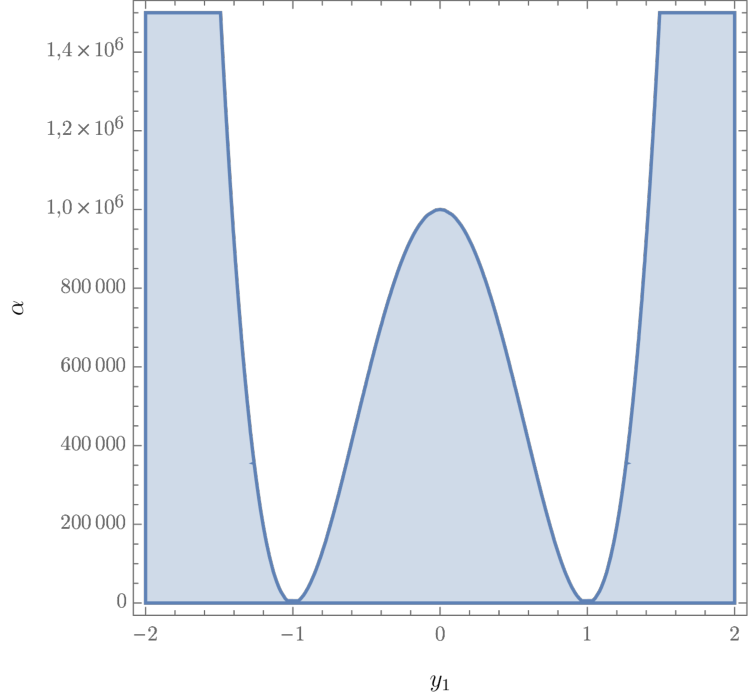
\includegraphics[width=0.8\textwidth]{1}
	\caption{}
	\label{fig:1}
\end{figure}
От $y_2$, как мы выяснили, жёсткость системы не зависит.
%Для случая комплексно-сопряжённых корней
%выбор $\lambda$ не ограничен сверху, следовательно
%при $1<x\le 1$ коэффициент жёсткости
%так же можно выбрать равным нулю.
%
%Всё это как-то странно получается\ldots
%И тогда условие жёсткости системы запишется как
%\[
%\frac{\Lambda}{\lambda}\le \frac{x+\sqrt{x^2-1} }{x-\sqrt{x^2-1} }\ll 1
%.\] 
%\[
%\frac{x-\sqrt{x^2-1} }{x+\sqrt{x^2-1} }=2 x \left(x-\sqrt{x^2-1}\right)-1\ll 1
%.\] 
%Полученная для оценки функция --- положительная и строго-убывающая на промежутке
%$\left( -\infty,\,-1 \right] $ и в точке $x=-1$ равна единице,
%следовательно необходимое условие жёсткости
%Видно, что это условие тем лучше выполнено, чем ближе
%$x$ к -1. Раскладываясь по Тейлору в данной окрестности,
%получим
%или для переменной $y_1$:
%\[
%1000 \left(1-y_1^2\right) \left(-500 \left(y_1^2-1\right)-\sqrt{500^2
%   \left(y_1^2-1\right){}^2-1}\right)-1\ll 1
%.\] 
%\[
%x\pm \sqrt{x^2-1} \le 0 \implies x \le  \mp \sqrt{x^2-1} 
%.\] 
%Задача распадается на два случая:
%\begin{enumerate}
%\item Пусть
%\[
%	\lambda_1=500(1-y_1^2)+ \sqrt{500^2(1-y_1^2)^2-1} 
%,\]
%\[
%	\lambda_2=500(1-y_1^2)- \sqrt{500^2(1-y_1^2)^2-1} 
%.\]
%\end{enumerate}
\end{sol}
\begin{hiProb}[7.2]
Получить функции устойчивости всех явных методов Рунге–Кутты с порядком аппроксимации с первого до седьмого с минимальным числом стадий.
\end{hiProb}
\begin{sol}
Так как
\[
u_{n+1}=e^{\lambda h} u_n,\quad y_{n+1}=
R(\lambda h) y_n,\quad |u_{n+1}-y_{n+1}|=O\left(h^{p+1}\right)=
O\left(z^{p+1}\right)
,\] 
где $\lambda h=z$, то у $R(z)$ и $e^z$ ряды Тейлора
совпадают вплоть до порядка аппроксимации $p$.
Известно, что для $p\le 4$ существуют ЯМРК
с числом стадий $s=p$.

Для $p$ от 1 до 4 найдутся  $s$-стадийные методы
с числом стадий равным порядку аппроксимации,
значит для таких методов функция устойчивости
$R(z)$ не будет зависеть от конкретного вида
таблицы Бутчера и будет равна
\[
	R (z)=1+z+\ldots+\frac{z^s}{s!},
\] 
Далее, после так называемого первого барьера Бутчера,
методы с $p\ge 5$ будут, как минимум $s+1$-стадийные:
\[
	p=5:\quad R(z)=1+z+ \frac{z^5}{5!}+ C_6 z^6,
\] 
\[
	p=6:\quad R(z)=1+z+\ldots+\frac{z^6}{6!}+
	C_7 z^7
,\] 
где $C_6$ и $C_7$ зависят от таблицы Бутчера.
После второго барьера Бутчера ($p\ge 7$) методы
будут как минимум $s+2$-стадийные:
\[
p=7:\quad	R(z)=1+z+\ldots+\ldots+\frac{z^7}{z!}+
	C_8 z^8 +C_9 z^9
,\]
где, как и раньше, $C_8$ и $C_9$ зависят от конкретного
вида таблицы Бутчера.
\end{sol}
\begin{hiProb}[7.3]
Вывести условия порядка для всех двухстадийных НМРК вплоть до четвертого.
\end{hiProb}
\begin{sol}
Задача решалась при помощи пакета Mathematica:

\begin{mmaCell}[moredefined={s, F, list1, list2, set},morepattern={h_, i_, j_, \#},morefunctionlocal={i, h, j, m, p}]{Input}
  s=2;
  F[h_,i_]:=f[\mmaSub{x}{n}+\mmaSub{c}{\mmaPat{i}}\mmaPat{h},\mmaSub{y}{n}+\mmaPat{h} \mmaUnderOver{\(\pmb{\sum}\)}{j=1}{s}\mmaSub{a}{\mmaPat{i},j}\mmaSub{k}{j}[\mmaPat{h}]]
  list1=CoefficientList[Normal[Series[
  \mmaSub{y}{n}+h \mmaUnderOver{\(\pmb{\sum}\)}{i=1}{s}\mmaSub{b}{i}f[\mmaSub{x}{n}+\mmaSub{c}{i}h,\mmaSub{y}{n}+h\mmaUnderOver{\(\pmb{\sum}\)}{j=1}{s}\mmaSub{a}{i,j}\mmaSub{k}{j}[h]],\{h,0,4\}]]//.\{
  Derivative[i_][\mmaSub{k}{j_}][_] \(\pmb{\to}\)Derivative[\mmaUnd{i},0][F][0,\mmaUnd{j}],
  \mmaSub{k}{i_}[0]\(\pmb{\to}\)f[\mmaSub{x}{n},\mmaSub{y}{n}]\},\mmaUnd{h}];
  list2=CoefficientList[Normal[Series[
  u[\mmaSub{x}{n}+h],\{h,0,4\}]]
  //.Derivative[i_][u][_] \(\pmb{\to}\)  
  D[f[\mmaSub{x}{n},u[\mmaSub{x}{n}]],\{\mmaSub{x}{n},\mmaUnd{i}-1\}]/.u[\mmaSub{x}{n}]\(\pmb{\to}\)\mmaSub{u}{n},\mmaUnd{h}];
  set=Table[Derivative[m,p][f][\mmaSub{x}{n},\mmaSub{u}{n}],
  \{m,0,3\},\{p,0,3-m\}]//Flatten;
  Map[#==0&,DeleteCases[CoefficientList[
  #,set]&/@Flatten[\{list1-list2//Thread\}/.\mmaSub{y}{n}\(\pmb{\to}\)\mmaSub{u}{n}
  ],0,\mmaDef{\(\pmb{\infty}\)}]//Flatten]//Simplify
\end{mmaCell}

\begin{mmaCell}[addtoindex=5]{Output}
  \{\mmaSub{b}{1}+\mmaSub{b}{2}==1,2 \mmaSub{b}{1} \mmaSub{c}{1}+2 \mmaSub{b}{2} \mmaSub{c}{2}==1,2 \mmaSub{b}{1} (\mmaSub{a}{1,1}+\mmaSub{a}{1,2})+2
\mmaSub{b}{2} (\mmaSub{a}{2,1}+\mmaSub{a}{2,2})==1,3 \mmaSub{b}{1} \mmaSubSup{c}{1}{2}+3 \mmaSub{b}{2} \mmaSubSup{c}{2}{2}==1,6 \mmaSub{b}{1} (\mmaSub{c}{1}
\mmaSub{a}{1,1}+\mmaSub{c}{2} \mmaSub{a}{1,2})+6 \mmaSub{b}{2} (\mmaSub{c}{1} \mmaSub{a}{2,1}+\mmaSub{c}{2} \mmaSub{a}{2,2})==1,3 \mmaSub{b}{1} \mmaSub{c}{1}
(\mmaSub{a}{1,1}+\mmaSub{a}{1,2})+3 \mmaSub{b}{2} \mmaSub{c}{2} (\mmaSub{a}{2,1}+\mmaSub{a}{2,2})==1,6 \mmaSub{b}{1} (\mmaSubSup{a}{1,1}{2}+\mmaSub{a}{1,1}
\mmaSub{a}{1,2}+\mmaSub{a}{1,2} (\mmaSub{a}{2,1}+\mmaSub{a}{2,2}))+6 \mmaSub{b}{2} (\mmaSub{a}{1,1} \mmaSub{a}{2,1}+\mmaSub{a}{1,2} \mmaSub{a}{2,1}+\mmaSub{a}{2,2}
(\mmaSub{a}{2,1}+\mmaSub{a}{2,2}))==1,3 \mmaSub{b}{1} \mmaSup{(\mmaSub{a}{1,1}+\mmaSub{a}{1,2})}{2}+3 \mmaSub{b}{2} \mmaSup{(\mmaSub{a}{2,1}+\mmaSub{a}{2,2})}{2}==1,4
\mmaSub{b}{1} \mmaSubSup{c}{1}{3}+4 \mmaSub{b}{2} \mmaSubSup{c}{2}{3}==1,8 \mmaSub{b}{1} \mmaSub{c}{1} (\mmaSub{c}{1} \mmaSub{a}{1,1}+\mmaSub{c}{2}
\mmaSub{a}{1,2})+8 \mmaSub{b}{2} \mmaSub{c}{2} (\mmaSub{c}{1} \mmaSub{a}{2,1}+\mmaSub{c}{2} \mmaSub{a}{2,2})==1,12 (\mmaSub{b}{1} (\mmaSubSup{c}{1}{2}
\mmaSub{a}{1,1}+\mmaSubSup{c}{2}{2} \mmaSub{a}{1,2})+\mmaSub{b}{2} (\mmaSubSup{c}{1}{2} \mmaSub{a}{2,1}+\mmaSubSup{c}{2}{2} \mmaSub{a}{2,2}))==1,\mmaSub{b}{1}
(\mmaSub{c}{1} (\mmaSubSup{a}{1,1}{2}+\mmaSub{a}{1,2} \mmaSub{a}{2,1})+\mmaSub{c}{2} \mmaSub{a}{1,2} (\mmaSub{a}{1,1}+\mmaSub{a}{2,2}))+\mmaSub{b}{2}
(\mmaSub{c}{1} \mmaSub{a}{2,1} (\mmaSub{a}{1,1}+\mmaSub{a}{2,2})+\mmaSub{c}{2} (\mmaSub{a}{1,2} \mmaSub{a}{2,1}+\mmaSubSup{a}{2,2}{2}))==\mmaFrac{1}{24},4
\mmaSub{b}{1} \mmaSubSup{c}{1}{2} (\mmaSub{a}{1,1}+\mmaSub{a}{1,2})+4 \mmaSub{b}{2} \mmaSubSup{c}{2}{2} (\mmaSub{a}{2,1}+\mmaSub{a}{2,2})==1,8 \mmaSub{b}{1}
(\mmaSub{a}{1,1}+\mmaSub{a}{1,2}) (\mmaSub{c}{1} \mmaSub{a}{1,1}+\mmaSub{c}{2} \mmaSub{a}{1,2})+8 \mmaSub{b}{2} (\mmaSub{a}{2,1}+\mmaSub{a}{2,2})
(\mmaSub{c}{1} \mmaSub{a}{2,1}+\mmaSub{c}{2} \mmaSub{a}{2,2})==1,\mmaSub{b}{1} (\mmaSub{c}{2} \mmaSub{a}{1,2} (\mmaSub{a}{2,1}+\mmaSub{a}{2,2})+\mmaSub{c}{1}
(2 \mmaSubSup{a}{1,1}{2}+2 \mmaSub{a}{1,1} \mmaSub{a}{1,2}+\mmaSub{a}{1,2} (\mmaSub{a}{2,1}+\mmaSub{a}{2,2})))+\mmaSub{b}{2} (\mmaSub{c}{1} (\mmaSub{a}{1,1}+\mmaSub{a}{1,2})
\mmaSub{a}{2,1}+\mmaSub{c}{2} (\mmaSub{a}{1,1} \mmaSub{a}{2,1}+\mmaSub{a}{1,2} \mmaSub{a}{2,1}+2 \mmaSub{a}{2,2} (\mmaSub{a}{2,1}+\mmaSub{a}{2,2})))==\mmaFrac{5}{24},\mmaSub{b}{2}
(\mmaSubSup{a}{1,1}{2} \mmaSub{a}{2,1}+\mmaSub{a}{1,1} \mmaSub{a}{2,1} (\mmaSub{a}{1,2}+\mmaSub{a}{2,2})+\mmaSubSup{a}{2,2}{2} (\mmaSub{a}{2,1}+\mmaSub{a}{2,2})+\mmaSub{a}{1,2}
\mmaSub{a}{2,1} (\mmaSub{a}{2,1}+2 \mmaSub{a}{2,2}))+\mmaSub{b}{1} (\mmaSubSup{a}{1,1}{3}+\mmaSubSup{a}{1,1}{2} \mmaSub{a}{1,2}+\mmaSub{a}{1,1} \mmaSub{a}{1,2}
(2 \mmaSub{a}{2,1}+\mmaSub{a}{2,2})+\mmaSub{a}{1,2} (\mmaSub{a}{1,2} \mmaSub{a}{2,1}+\mmaSub{a}{2,2} (\mmaSub{a}{2,1}+\mmaSub{a}{2,2})))==\mmaFrac{1}{24},4
\mmaSub{b}{1} \mmaSub{c}{1} \mmaSup{(\mmaSub{a}{1,1}+\mmaSub{a}{1,2})}{2}+4 \mmaSub{b}{2} \mmaSub{c}{2} \mmaSup{(\mmaSub{a}{2,1}+\mmaSub{a}{2,2})}{2}==1,3
\mmaSub{b}{2} (\mmaSubSup{a}{1,1}{2} \mmaSub{a}{2,1}+\mmaSubSup{a}{1,2}{2} \mmaSub{a}{2,1}+2 \mmaSub{a}{1,2} \mmaSub{a}{2,1} (\mmaSub{a}{2,1}+\mmaSub{a}{2,2})+3
\mmaSub{a}{2,2} \mmaSup{(\mmaSub{a}{2,1}+\mmaSub{a}{2,2})}{2}+2 \mmaSub{a}{1,1} \mmaSub{a}{2,1} (\mmaSub{a}{1,2}+\mmaSub{a}{2,1}+\mmaSub{a}{2,2}))+3
\mmaSub{b}{1} (3 \mmaSubSup{a}{1,1}{3}+6 \mmaSubSup{a}{1,1}{2} \mmaSub{a}{1,2}+\mmaSub{a}{1,2} (\mmaSub{a}{2,1}+\mmaSub{a}{2,2}) (2 \mmaSub{a}{1,2}+\mmaSub{a}{2,1}+\mmaSub{a}{2,2})+\mmaSub{a}{1,1}
\mmaSub{a}{1,2} (3 \mmaSub{a}{1,2}+2 (\mmaSub{a}{2,1}+\mmaSub{a}{2,2})))==1,4 \mmaSub{b}{1} \mmaSup{(\mmaSub{a}{1,1}+\mmaSub{a}{1,2})}{3}+4 \mmaSub{b}{2}
\mmaSup{(\mmaSub{a}{2,1}+\mmaSub{a}{2,2})}{3}==1\}
\end{mmaCell}
\end{sol}
\begin{hiProb}[7.4]
Для системы ОДУ
\[
	\dot{x}_1=98 x_1+198 x_2,\\
	\dot{x}_2=-99x_1 -199 x_2
\]
численное решение задачи Коши с начальными данными
\[
	x_1(0)=1,\quad x_2 (0)=1
\]
получают явными методами Рунге-Кутты 1,2,3 и 4 порядков
аппроксимации с числом стадий, равным порядку аппроксимации.
При каких шагах $\tau$ каждый из методов устойчив?
Объяснить, почему для методов с числом стадий и 3
и с числом стадий 2 и 4 развитие неустойчивости
носит качественно различный характер.
\end{hiProb}
\begin{sol}
Матрица данной системы ОДУ
\[
	A= \begin{pmatrix} 98 & 198 \\ -99
	& -199\end{pmatrix} 
\] 
имеет собственные значения
\[
\lambda_1=-1,\quad \lambda_2=-100
.\] 
Так как оба собственных значения --- вещественные,
то функция устойчивости $R(z)$ также вещественная.
Для исследуемых методов Рунге-Кутты
\[
	R(z)= \sum_{n=0}^{p} \frac{z^n}{n!},\quad
	z=\lambda \tau
.\] 
%Имеется два собственных значения: $\lambda_1$ и
%$\lambda_2$. 
\begin{enumerate}
\item $p=1$:
	\[
		|R(z)|=|1+z|\le 1 \Leftrightarrow
		-2 \le  z\le 0
	.\] 
	\[
	\left\{
	\begin{aligned}
	\tau \le 2 /\lambda_1\\
	\tau \le  2 /\lambda_2
	\end{aligned}
	\right.
	\implies \tau\le 0,02
	.\] 
\item $p=2$:
	\[
		|R(z)|=\left| 
		1+z+ \frac{z^2}{2}\right| \le 1
	.\] 
	\[
	-2 \le z \le 0 \implies \tau \le 0
	.\] 
\item $p=3$:
	\[
		|R(z)|=\left| 1+z+\frac{z^2}{2}+
		\frac{z^3}{6}\right| \le 1 \implies
		-2,513\le z\le 0
	.\] 
	\[
	\tau\le 0,025
	.\] 
\item $p=4$:
	\[
		|R(z)|= \left| 
		1+z + \frac{z^2}{2}+
		\frac{z^3}{6}+ \frac{z^4}{24}\right| \le 1 \implies -2,785\le z\le 0
	.\] 
	\[
	\tau \le 0,027
	.\] 
\end{enumerate}
Характер неустойчивости:
\begin{enumerate}
	\item Для 1 и 3 порядка $R(z)<-1$ при $\tau
		>\tau_\text{гр}$, $y_{n+1}=
		R(z)y_n$; $y_0=1 \implies$
		будут происходить
		осцилляции с увеличивающейся
		амплитудой до
		бесконечности
	\item Для 2 и 4 порядка $R(z)>1\implies$
		нет осцилляций, поэтому
		монотонный неограниченный
		рост.
\end{enumerate}
\end{sol}
\begin{hiProb}[7.5]
Рассматривается следующее параметрическое семейство
однократно диагонально-неявных методов Рунге-Кутты (табл.~\ref{tab:1}).
\begin{table}[htpb]
\centering
\caption{}
\label{tab:1}
\begin{tabular}{Cc|CcCc}
	$\gamma$ & $\gamma$ &  \\
	$1-\gamma$ & $1-2\gamma$ & $\gamma$ \\
	 \hline& $\frac{1}{2}$ & $\frac{1}{2}$ \\
\end{tabular}
\end{table}
Найти все значения параметра, при которых
\begin{enumerate}
\item метод имеет третий порядок аппроксимации;
\item метод является асимптотически устойчивм;
\item метод является $A$-устойчивым.
\end{enumerate}
\end{hiProb}
\begin{sol}
\begin{enumerate}
	\item 
\begin{itemize}
\item $\displaystyle  \sum_{i=1}^{2} b_i= \frac{1}{2}+\frac{1}{2}=1$ --- первый порядок;
\item $\displaystyle \sum_{i=1}^{2} b_i c_i=
	\frac{\gamma}{2}+\frac{1}{2}-\frac{\gamma}{2}=\frac{1}{2}$ --- второй порядок;
\item $\displaystyle \sum_{i=1}^{2} b_i c_i^2=
	\frac{\gamma^2}{2}+ \frac{\gamma^2-2\gamma
	+1}{2}=\gamma^2-\gamma +\frac{1}{2}=\frac{1}{3}$;

	$\displaystyle 
	\sum_{i=1}^{2} b_i \sum_{j=1}^{2} a_{ij}
	c_j= \gamma-\gamma^2=\frac{1}{6}$;
	\[
	\left\{
	\begin{aligned}
	\gamma^2-\gamma+\frac{1}{6}&= 0 \\
	\gamma^2-\gamma+\frac{1}{6}&= 0 \\
	\end{aligned}
	\right.
	\implies \gamma_{1,2}=
	\frac{1\pm \sqrt{1-\frac{2}{3}} }{2}=
	\frac{1}{2}\pm \frac{1}{2 \sqrt{3} }
	\] --- третий порядок при $\displaystyle \gamma=\frac{1}{2}\pm \frac{1}{2 \sqrt{3} }$. 
\end{itemize}
\item $\displaystyle R(z)= \frac{\det \left( 
	\mathbf{E}-z\mathbf{A}+z \mathbf{e}
	\mathbf{b}^T\right) }{\det
(\mathbf{E}-z \mathbf{A})}=\frac{z (-4 \gamma +2 (\gamma -2) \gamma  z+z+2)+2}{2 (\gamma  z-1)^2}$
\[
\lim_{\Re z \to -\infty} =1-\frac{1}{2\gamma^2}-
\frac{2}{\gamma}=0\implies
2\gamma^2-4\gamma +1=0
.\] 
\[
\gamma_{1,2}= 1\pm \frac{\sqrt{2} }{2}
.\] 
\item \[
\left\{
\begin{aligned}
	|R(z)|\le 1\\
	\Re  z\le 0
\end{aligned}
\right.
\implies \gamma \ge \frac{1}{4}
.\] 
\end{enumerate}
\end{sol}
\begin{hiProb}[7.12]
	Исследовать на $A(\alpha)$-устойчивость
	схему:
	\[
	4 \frac{y_{n+1}-y_{n-1}}{2h}-
	3 \frac{y_{n+1}-y_n}{h}=f_n
	.\] 
\end{hiProb}
\begin{sol}
\[
4 \frac{y_{n+1}-y_{n-1}}{2h}-3 \frac{y_{n+1}-y_n}{h}=f_n=\lambda y_n
.\] 
\[
2y_{n+1}-2y_{n-1}- 3 y_{n+1}+3 y_n=zy_n
.\] 
\[
	y_{n+1}-(3-z)y_n+2 y_{n-1}=0
.\] 
\[
	y_{n+1}=R(z)y_n=R^2(z)y_{n-1}
.\] 
\[
	R^2(z)-(3-z)R(z)+2=0\implies
	R_{1,2}(z)= \frac{3-z \pm \sqrt{z^2-6z+1} }{2}
.\] 
Области
\[
	|R_1(z)|\le 1 \text{ и } |R_2(z)|\le 1
\]
представлены на рис.~\ref{fig:2}.
\begin{figure}[htpb]
	\centering
	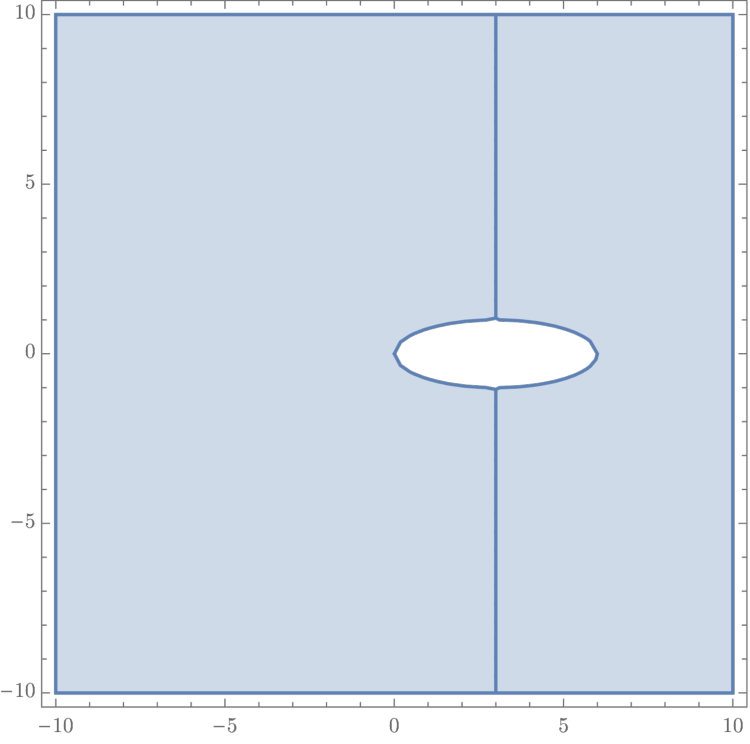
\includegraphics[width=0.8\textwidth]{2}
	\caption{}
	\label{fig:2}
\end{figure}
Они не пересекаются, следовательно исследуемая схема
не $A(\alpha)$-устойчива.
\end{sol}
\begin{hiProb}[7.16]
Исследовать на аппроксимацию метод решения задачи Коши
для ЖС ОДУ (табл.~\ref{tab:2}).
\begin{table}[htpb]
\centering
\caption{}
\label{tab:2}
\begin{tabular}{Cc|CcCc}
	$-\sqrt{2} /2$ & $-\sqrt{2} /2$ &  \\
	$1 /2-\sqrt{2} /2$ & $-1 /2$ & $1-\sqrt{2} /2$ \\
	 \hline& $\sqrt{2} $ & $1-\sqrt{2} $ \\
\end{tabular}
\end{table}
При необходимости внести изменения в таблицу Бутчера для
повышения порядка аппроксимации метода. Определить
тип устойчивости на действительной оси модифицированной
схемы.
\end{hiProb}
\begin{sol}
Условие порядка не ниже первого 
 \[
 \sum_{i=1}^{2} b_i=1
\]
выполнено. Условие по крайней мере второго порядка аппроксимации:
\[
\sum_{i=1}^{2} b_i c_i= \frac{1}{2}-\sqrt{2} \neq \frac{1}{2}
\] 
не выполнено, следовательно порядок аппроксимации метода $p=1$.
Для повышения порядка аппроксимации метода до второго, необходимо заменить
\[
	c_{22}\to -\frac{3}{2}\left( 1+\sqrt{2}  \right) 
.\] 
Тогда последнее условие будет также выполнено. 
\[
R(z)= \frac{\det \left( 
	\mathbf{E}-z\mathbf{A}+z \mathbf{e}
	\mathbf{b}^T\right) }{\det
(\mathbf{E}-z \mathbf{A})}=
-\frac{\left(\sqrt{2}-2\right) z^2+2 \left(1+\sqrt{2}\right)
   z+2}{\left(\sqrt{2}-1\right) (z-2) z-2}
.\] 
Условие
\[
	|R(z)|\le 1
\]
будет выполнено при
\[
2 \sqrt{2}-2 \sqrt{3}\leq z\leq 0\text{ или } 2 \sqrt{2}+2 \sqrt{3}\leq z\leq
   -\frac{4}{2 \sqrt{2}-3}
.\] 
Значит на этих промежутках метод абсолютно устойчив.
\end{sol}
\begin{hiProb}[7.19]
Исследовать свойства монотонности следующих схем:
\renewcommand{\labelenumi}{\asbuk{enumi})}
\begin{enumerate}
\item формулы трапеций,
\item явной и неявной схем Эйлера,
\item схемы Розенброка с комплексными коэффициентами.
\end{enumerate}
\end{hiProb}
\begin{sol}
\renewcommand{\labelenumi}{\asbuk{enumi})}
\begin{enumerate}
\item Формула метода трапеции:
	\[
	\frac{y_{n+1}-y_n}{h}=\frac{1}{2}
	\left( f(x_n,\,y_n)+
	f(x_{n+1},\,y_{n+1})\right) 
	.\] 
	С учётом уравнения Далквиста
	\begin{multline*}
	y_{n+1}=y_n+\frac{h\lambda}{2}y_n+
	\frac{h\lambda}{2}y_{n+1}\implies
	y_{n+1}\left( 1-\frac{z}{2} \right) =\\=
	y_n \left( 1+\frac{z}{2} \right) \implies
	y_{n+1}=y_n \left( 
	\frac{2+z}{2-z}\right) \implies
	R(z)=\frac{2+z}{2-z}
	.\end{multline*} 
	Видим, что на отрицательной части
	действительной оси $R(z)$ не
	всегда положительна, значит
	схема трапеции не 
	является монотонной.
\item Для явной и неявной схем Эйлера известно, что
	 \[
		 R(z)=1+z,\quad R(z)=\frac{1}{1-z}
	\]
	соответственно. Легко видеть, что
	первая  не будет монотонной, а
	вторая будет.
\item Для CROS
	 \[
		 R(z)= \frac{1}{1-z+\frac{z^2}{2}}
	.\] 
	Схема будет монотонной, поскольку на
	отрицательной части действительной оси
	знаменатель $R(z)$ положительный.
\end{enumerate}
\end{sol}
\begin{hiProb}[8.8]
Выберите значение $y_1$ таким образом, чтобы
соответствующее решение разностного уравнения
\[
	y_{n+1}=y_{n-1}+2h(-2y_n+1)
\]
с $y_0=1$ стремилось к нулю при $n\to \infty$. Составьте
программу, реализующую численное решение уравнения
как с найденным значением $y_1$, так и со значением
$y_1$, задаваемым формулой $y_1=0.5 e^{-2h}+0.5$.
Проанализируйте получающиеся результаты.
\end{hiProb}
\begin{sol}
Для однородной задачи можем записать
\[
y_{n+1}-4 h y_n-y_{n-1}=0
.\] 
\[
q^2+4 h q-1=0
.\] 
\[
q_{1,2}=-2h\pm \sqrt{4h^2+1} 
.\] 
\[
|q_1|<1,\quad q_1 >0,\quad |q_2|>1,\quad
q_2 <0
.\] 
Общее решение разностной задачи можем записать как
\[
y_n=\alpha q_1^n +\beta q_2^n +\frac{1}{2}
.\] 
\[
y_0=\alpha+\beta +\frac{1}{2}=1 \implies
\alpha+\beta =\frac{1}{2}
.\] 
Чтобы решение сходилось к $\frac{1}{2}$ нужно
положить $\beta=0$, $\alpha=\frac{1}{2}$, тогда
\[
	y_n=\frac{1}{2}\left(q_1^n+1\right)
.\] 
\[
	y_1=\frac{1}{2} \left( 
	1-2h +\sqrt{4h^2 +1} \right) 
.\] 
Если же исходить из заданного изначально
$y_1= 0.5 e^{-2h}+0.5$, получим
\[
	y_1=\left( \frac{1}{2}-\beta \right) q_1+ \beta q_2 +\frac{1}{2}= \frac{1}{2}\left( e^{-2h}+1 \right) 
.\] 
Откуда
\[
\beta=\frac{e^{-2 h} \left(e^{2 h} q_1-1\right)}{2 \left(q_1-q_2\right)}=
\frac{\sqrt{4 h^2+1}-2 h-e^{-2 h}}{4 \sqrt{4 h^2+1}}
=\frac{h^3}{3}+O(h^4)\neq 0
.\] 
Следовательно, решение, построенное данным
методом будет расходиться.

Реализация обоих методов в пакете Mathematica:
\begin{mmaCell}[moredefined={h,ListLinePlot},morepattern={i_, n_, i, n}]{Input}
  \mmaSub{y}{1,0}=1.;
  h=.01;
  \mmaSub{y}{1,1}=\mmaFrac{1}{2}(1-2 h+\mmaSqrt{1+4 \mmaSup{h}{2}});
  \mmaSub{y}{2,1}=0.5+0.5\mmaSup{\mmaDef{e}}{-2h};
  \mmaSub{y}{i_,n_}:=\mmaSub{y}{i,n}=\mmaSub{y}{i,n-2}+2.h(-2.\mmaSub{y}{i,n-1}+1.)
  ListLinePlot[Table[\{h \mmaFnc{n},\mmaSub{y}{\mmaFnc{i},\mmaFnc{n}}\},\{\mmaFnc{i},2\},\{\mmaFnc{n},0,100\}]]
\end{mmaCell}
\begin{mmaCell}[moregraphics={moreig={scale=.7}}]{Output}
\mmaGraphics{3}
\end{mmaCell}
%
%Переписав разностное уравнение в виде
%	\[
%	\frac{y_{n+1}-y_{n-1}}{2h}=1-2y_n
%	\] 
%можем заметить, что это метод Эйлера с центральной точкой 
%для дифференциальной задачи
%\[
%u'=1-2u
%.\] 
%Общее решение
%	\[
%		q^2=1+2h(-2q+1)
%	.\] 
%\[
%	y_2=y_0+2h(-2y_1+1)
%.\] 
%\[
%	y_3=y_1+2h(
%.\] 
%\ldots
\end{sol}
\section*{Тема XI. Численное решение ОДУ: краевые
	задачи}	
\begin{hiProb}[7.2]
Для численного отыскания периодического с периодом
единица решения уравнения
\[
	y''+p(x)y'+q(x)y=f(x)
,\] 
где $f,\,q,\,p$ --- заданные функции, используется
разностная схема второго порядка аппроксимации с центральной
разностью
\[
\frac{y_{n+1}-2y_n+y_{n-1}}{h^2}+
p_n \frac{y_{n+1}-y_{n-1}}{2h}+q_n y_n=f_n
.\] 
Предложить модификацию метода прогонки
(периодическая прогонка) для решения данной задачи.
\end{hiProb}
\begin{sol}
Рассмотрим следующую краевую задачу для уравнения:
\[
	y''+p(x)y'+q(x) y=f(x)
\] 
с условиями периодичности
\[
	y ^{(p)}(0)=y^{(p)} (1)
,\]
где $p$ принимает значения 0 и 1.

Краевая задача с условиями периодичности решается
методом циклической прогонки. Запишем дискретный
аналог уравнения:
 \[
\frac{y_{n+1}-2y_n +y_{n-1}}{h^2}+p_n
\frac{y_{n+1}-y_{n-1}}{2h}+q_n y_n=f_n
.\] 
Очевидно, что оно аппроксимирует дифференциальную задачу
со вторым порядком на равномерной сетке. На случай
неравномерной сетки рассматриваемый метод легко
обобщается.

В силу периодичности дискретное уравнение должно
выполняться во всех точках сетки, включая граничные.
Кроме того, в силу граничного условия при $p=0$ 
$y_0=y_{N+1}$. Система сеточных соотношений примет вид
\[
a_0 y_N-b_0 y_0+c_0y_1=\phi_0,
\] 
\[
\ldots
\] 
\[
	a_n y_{n-1}-b_n y_n +c_n y_{n+1}=\phi_n
\] 
\[
\ldots
\] 
\[
a_{N}y_{N-1} -b_N y_N +c_N y_0= \phi_N
,\] 
где $a_k=1-0.5 p_k h$, $b_k=2-q_k h^2$, $c_k=1+0.5p_k h$,
$\phi_k =f_k h^2$. Матрица системы линейных
уравнений получается <<почти трёхдиагональной>> ---
от трёхдиагональной её отличают всего два элемента
в углах матрицы.

Обобщение стандартных прогоночных соотношений 
(для трёхточечной прогонки) на периодический случай
будет иметь вид
\[
y_{n-1}=\alpha_n y_n +\beta_n \gamma_n y_N
.\] 
Из приведённого выше соотношения для $y_0$ сразу
получаем, что
\[
\alpha_1 = \frac{c_0}{b_0},\quad
\beta_1= - \frac{\phi_0}{b_0},\quad
\gamma_1= \frac{a_0}{b_0}
.\] 
Теперь несложно получить рекуррентную зависимость
для прогоночных коэффициентов:
\[
a_{k+1}= \frac{c_k}{b_k-\alpha_k a_k},\quad
\beta_{k+1} = \frac{a_k \beta_k -\phi_k}{b_k-\alpha_k
a_k},\quad \gamma_{k+1}= \frac{a_k \gamma_k}{b_k -\alpha_k
a_k}
.\]
По приведённым выше формулам получаются значения
коэффициентов для всех уравнений с номерами меньше,
чем $N$. Это уже известный прямой ход прогонки слева
направо.

Подставим теперь прогоночные соотношения в последнее
уравнение линейной системы. В итоге с учётом
введённых выше обозначений получаем
\[
	a_N \left( \alpha_N y_N+\beta_N+\gamma_N
	y_N\right) -b_N y_N+c_N y_0=\phi_N
,\] 
а это соотношение, сгруппировав члены, можно 
переписать как
\[
y_N=\mu_N y_0 +\nu_N
,\] 
где введены обозначеения
\[
	\mu_N= \frac{-c_N}{a_N \left( \alpha_N+ \gamma_N \right) -b_N},\quad \nu_N= \frac{\phi_N -a_N
	\beta_N }{a_N \left(  \alpha_N +\gamma_N\right)-b_N }
.\] 
Теперь выражение для значения сеточной функции
$y_{n-1}$ подставляем в прогоночные соотношения.
Получается выражение,  связывающее $y_{n-1}$ с
$y_0$:
\[
	y_{n-1} =\alpha_n \left( \mu_n y_0 +\nu_n \right) +
	\beta_n +\gamma_n \left( \mu_N y_0 +\nu_N \right) 
.\] 
Отсюда получаем следующие рекуррентные соотношения:
\[
\mu_{n-1}=\alpha_n \mu_n +\gamma_n \mu_N,\quad
\nu_{n-1}=\beta_n+\alpha_n \nu_n +\gamma_n \nu_N
.\] 
Отметим, что эти коэффициенты вычисляются в обратном
порядке справа налево --- аналог обратного хода
прогонки. Последнее соотношение  приводит к явному
выражению для $y_0$. В результате получаем
\[
y_0= \frac{\nu_0}{1-\mu_0}
.\] 
Теперь информации для определения значений искомой функции
во всех точках сетки (ещё один ход прогонки) достаточно.
\end{sol}
\begin{hiProb}[8.1]
Описать алгоритм численного построения общего решения
для следующих дифференциальных уравнений:
\renewcommand{\labelenumi}{\asbuk{enumi})}
\begin{enumerate}
	\item $y''-(10+x)y=z e^{-x}$, $0<x<10$;
	\item $y''+(10+x)y=x e^{-x}$, $0<x<10$.
\end{enumerate}
\end{hiProb}
\begin{sol}
Имеем уравнение:

$$
y'' \mp (10+x)y = x e^{-x},\;\; 0< x< 10.
$$

Представим решение в виде:

$$
y = C_1 y_1 + C_2 y_2 + y_3.
$$

Где $y_1,\; y_2$ --- решения задачи Коши для однородного уравнения:
\begin{gather*}
y''_1 \mp (10+x) y_1 =0\\
y_1(0) = 1,\\
y_1(10) = 0.
\end{gather*}
\begin{gather*}
y''_2 \mp (10+x) y_2 = 0\\
y_2(0) = 0,\\
y_2(10) = 1.
\end{gather*}
А $y_3$ $-$ частное решение:
\begin{gather*}
y''_3 \mp (10+x) y_3 = x e^{-x},\\
y_3(0) = y_3(10) = 0.
\end{gather*}
Найдем общие решения:

Первое решение:

\begin{gather*}
\frac{y_{2} - 2y_1 + 1}{h^2} \mp (10+h) y_1 = 0\\
\frac{y_{n+1} - 2y_n + y_{n-1}}{h^2} \mp (10+x_n) y_n = 0\\
\frac{-2y_{N-1} + y_{N-2}}{h^2} \mp (10 + x_{N-1}) y_{N-1} = 0.
\end{gather*}
Тогда имеется матрица:

$$
\frac{1}{h^2} \begin{pmatrix}
-2 \mp (10+h)h^2 & 1 & 0 & \dots & 0 & 0\\
1 & -2 \mp (10 + x_2)h^2 & 1 & \dots & 0 & 0\\
\vdots & \vdots & \vdots & \ddots & \vdots & \vdots\\
0 & 0 & 0 & \dots & -2 \mp (10+x_{N-2})h^2 & 1\\
0 & 0 & 0 & \dots &  1 & -2 \mp (10+x_{N-1})h^2
\end{pmatrix}
$$
C вектором правой части

$$
f_1 = \frac{1}{h^2} (-1, 0,..., 0)^{T}.
$$

И мы решаем систему

$$
Ay = f_1.
$$

Здесь за $A$ обозначена матрица, выписанная выше. Если мы решаем задачу для $y_2$, то помеяется только вектор правой части на

$$
f_2 = \frac{1}{h^2} (0,...,0, -1)^{T}.
$$

А если решать для $y_3$, то, конечно тоже меняется только правая часть:

$$
f_3 = (x_1 e^{-x_1}, x_2 e^{-x_2},..., x_{N-1} e^{-x_{N-1}})^{T}.
$$

Как же решать эти системы? Матрицы являются трехдиагональными, поэтому достаточно использовать метод прогонки.
Заметим, что в системе имеется строгое диагональное преобладание:

$$
|2 + (10+h)h^2| > 2.
$$

Для знака "минус". К тому же

$$
P_1 = \frac{c_0}{b_0} = \frac{1}{2 + (10+h)h^2} <1.
$$

Поэтому метод устойчив.

В другом случае получается, что метод прогонки неустойчив, поэтому будем строить наши решения, решая не краевую задачу, а задачу Коши:
\begin{gather*}
y''_1 + (10-x)y_1 = 0,\\
y_1(0) = 0,\\
y'_1(0) = 1\\
\end{gather*}
\begin{gather*}
y''_2 + y_2(10-x) = 0,\\
y_2(0) = 1,\\
y'_2(0) = 0.
\end{gather*}
\begin{gather*}
y''_3 + y_3(10-x) = xe^{-x},\\
y_3(0) = y'_3(0) = 0.
\end{gather*}

Теперь можно перейти к форме системы:
\begin{gather*}
u' = v,\\
v' = -(t+10)u + t e^{-t}.
\end{gather*}
Якобиан этой системы:

$$
Df = \begin{pmatrix}
0 & 1\\
-(t+10) & 0
\end{pmatrix}
$$

Отсюда собственные числа:

$$
\lambda_\pm = \pm i\sqrt{t+10}.
$$

То есть траектории ограничены. Поэтому имеет смысл искать какой-то метод для решения этих задач. Чтобы решить каждую из систем можно воспользоваться, например, методами из прошлой темы.
\end{sol}
\begin{hiProb}[8.2в]
Используя метод Ньютона, найти следующее приближение
к решению краевой задачи:
\[
	y''+(y')^2-8 \exp (y-x) +23=0,\quad
	y(0)=0,\ y(1)=1
.\] 
В качестве начального приближения взять $y^0(x)=x$.
\end{hiProb}
\begin{sol}
Необходимо сделать подстановку
\[
	y=y^0(x)+v(x)
.\] 
Тогда получается
\[
\left(v'+1\right)^2+v''-8 e^{v}+23=0
.\] 
После лианеризации:
\[
2 v'+v''-8 v+16=0
.\] 
Так как нулевое приближение уже выполняет граничные
условия, то граничные условия на поправку имеют вид
\[
	v(0)=v(1)=0
.\] 
Собственно, само приближение:
\[
	y^1(x)=x+ \frac{2 \left(-e^{4-4 x}-\left(1+e^2\right) e^{2 x}+1+e^2+e^4\right)}{1+e^2+e^4}
.\] 
\end{sol}
\begin{hiProb}[8.3$^*$]
Найти наименьшее число $\lambda$, при котором
следующая задача имеет нетривиальное решение:
\[
\left\{
\begin{aligned}
	y''+(\lambda-x^2)y&= 0,\quad x \in [0,\,1] \\
	y(0)=y(1)&=0
\end{aligned}
\right.
.\] 
Найти начальное приближение для наименьшего собственного
значения и указать алгоритм его дальнейшего нахождения
с заданной точностью.
\end{hiProb}
\begin{sol}
Имеем задачу Коши:
$$
\begin{cases}
y'' + (a - x^2)y = 0,\;\; x\in [0, 1]\\
y(0) = y(1) = 0.
\end{cases}
$$
Хотим найти наименьшее $a$, при котором задача имеет решение. Давайте возьмем сетку с шагом $h$ и используем разностную схему второго порядка:
$$
\frac{y_{2} - 2y_{1}}{h^2} + (a - x_1^2) y_1 = 0\\
\frac{y_{n+1} - 2y_n + y_{n-1}}{h^2} + (a - x_n^2) y_n = 0\\
\frac{-2y_{N-1} + y_{N-2}}{h^2} + (a - x_{N-1}^2) y_{N-1} = 0.
$$
Эта система задается матрицей:

$$
\frac{1}{h^2} \begin{pmatrix}
-2 +(a - x_1^2)h^2 & 1 & 0 & \dots & 0 & 0\\
1 & -2 + (a - x_2^2)h^2 & 1 & \dots & 0 & 0\\
\vdots & \vdots & \vdots & \ddots & \vdots & \vdots\\
0 & 0 & 0 & \dots & -2 + (a - x_{N-2}^2)h^2 & 1\\
0 & 0 & 0 & \dots &  1 & -2 + (a-x_{N-1}^2)h^2
\end{pmatrix}
$$
С нулевой правой частью. Поэтому условие совместности выражается в виде условия

$$
\det A = 0.
$$

Таким образом, мы имеем уравнение, которое для произвольного $h$ в принципе можно выписать, но, казалось бы, лучше оставить эту идею, и работать с определителем, как с какой-то функцией, заданной таблицей --- мы умеем ее вычислять через методы линейной алгебры, например. Если же метод окажется слишком дорогим, то матрицу можно в целом сначала диагонализовать методом прогонки, а потом просто перемножить диагональные элементы --- скорее всего при очень больших шагах это будет существенно быстрее (предполагается, что нам понадобится большое число шагов, ведь арифметика конечна, поэтому ошибка округления может стать слишком большой).

Итак, на каждом фиксированном $h_i$ мы умеем считать $\det A(a)$. С помощью какого-нибудь метода Ньютона, где производные аппроксимированы значениями функции $\det A(a)$ или же, с помощью формулы производной определителя посчитаны напрямую, мы можем решать уравнение $\det A(a) = 0$, беря в качестве начального приближения $a$ с прошлого шага разбиения $h_{i-1}$. Так как определитель это просто многочлен все условия сходимости выполнены.

Теперь у нас имеется функция $a(h)$ на сетке по $h$. Ее можно интерполировать какими-то полиномами, например $x^i$, а шаг брать $h_k = 1/(k+1)$. Ожидаем регулярную функцию $a(h)$, поэтому в самом худшем случае должен сходиться ряд тейлора от этой функции. В таком случае, грубой оценкой можно ожидать, что

$$
\frac{\max |f^{(n+1)}(0)|}{(n+1)!} \to 0,\;\; n\to \infty.
$$

Что следует из необходимого условия сходимости. Понятно, что производная в нуле существенно определяет оценку по всему отрезку, так как если что-то пойдет не так на конце около $h=1$, то мы просто отдалимся от этого конца. В итоге ошибка для интерполяции будет равна

$$
E(h) = \frac{\max_h |a^{(n+1)}(h)|}{(n+1)!} \prod |h - h_k| \sim \prod |h - h_k| .
$$

В нуле же получается

$$
E(h) \sim \frac{1}{N!}.
$$

Подобный выбор многочленов $x^i$ автоматически зануляет функцию Лебега в нуле, поэтому можно считать, что погрешность задается $E(h)$.

Найдем первую итерацию, то есть решение при $k=1$:

$$
h = 1/2,\\
\begin{cases}
-2y_1 + (a - (1/2)^2) (1/2)^2 y_1 = 0
\end{cases}
$$
\end{sol}
\begin{hiProb}[8.4в,д]
\end{hiProb}
\begin{sol}
Работаем на отрезке зке [0, 100] и решаем системы

$$
\begin{cases}
x' =  8x + 8y + 6z,\\
y' = 2x -2y + 2z,\\
z' = -11x - 8y - 9z.
\end{cases}
$$

И 

$$
\begin{cases}
x' = 5x + 3y - 2z,\\
y' = 6x - 2y - 6z,\\
z' = 6x + 3y- 3z.
\end{cases}
$$

С матрицами соответственно

$$
A_1 = \begin{pmatrix}
8 & 8 & 6\\
2 & -2 & 2\\
-11 & -8 & -9
\end{pmatrix},\;\;\; A_2 = \begin{pmatrix}
5 & 3 & -2\\
6 & -2 & -6\\
6 & 3 & -3
\end{pmatrix}
$$
Диагонализуем первую. Видно, что имеются значения 

$$
\lambda = \pm 1,\;\; \lambda = 2.
$$

На масштабе $x\in [0, 100]$ у нас получается 1 быстрозатухающее решение и два быстрорастущих, поэтому надо задать 1 условие на левом конце и два на правом для наилучшей обусловленности системы.

Диагонализуем вторую матрицу.
Результат не поменялся, поэтому не поменяется и ответ:

Два условия справа и одно слева.
\end{sol}
\begin{hiProb}[8.5]
\end{hiProb}
\begin{sol}
Имеем задачу Коши:

$$
\frac{d}{dx}\left(k(x) \frac{d}{dx}u\right) - q(x) u = -f(x)\\
k(0)u'(0) = 0,\;\; -k(1)u'(1) = u(1).
$$

Тут введены обозначения:

$$
k(x) = e^x,\;\; q(x) = e^x,\;\; f(x) = \sin x.
$$
С учетом этих обозначений у нас получится задача Коши:

$$
\frac{d}{dx}\left(e^x u'\right) - e^x u = - \sin x
u'(0) = 0,\;\; -eu'(1) = u(1).
$$

Упростим уравнения, меняя правую часть:

$$
u'' + u' - u = - e^{-x} \sin x.\\
u'(0) = 0,\;\; u(1) + e u'(1) = 0.
$$
Теперь нам остается подставить какие-то разностные схемы второго порядка вместо всех производных:

$$
u' = \frac{u_{n+1} - u_{n-1}}{2h}\\
u'' = \frac{u_{n+1} - 2u_{n} + u_{n-1}}{h^2}
$$

Такой подход создает некоторые проблемы с фиктивными узлами $y_{-1}$ и $y_{N+1}$, которые мы сейчас обработаем.

Cначала посмотрим на левый конец:

$$
\frac{y_{-1} - y_{1}}{h^2} = 0.
$$

$$
\frac{y_{1} - 2 y_0 + y_{-1}}{h^2} + \frac{y_1 - y_{-1}}{2h} - y_0 = 0.
$$

Система позволяет выразить $y_{-1}$, поэтому расширение схемы на этот фиктивный узел не испортит совместности.
Теперь правый конец:

$$
y_N + e \frac{y_{N+1} - y_{N-1}}{2h} = 0.
$$

$$
\frac{y_{N+1} - 2y_N + y_{N-1}}{h^2} + \frac{y_{N+1}-y_{N-1}}{2h} - y_N = - e^{-1}\sin (1).
$$

Внутренние точки получаются равны:

$$
\frac{y_{n+1} - 2y_n + y_{n-1}}{h^2} + \frac{y_{n+1} - y_{n-1}}{2h} + y_n = - e^{x_n} \sin x_n.
$$

\end{sol}
\begin{hiProb}[9.1а]
\end{hiProb}
\begin{sol}
Имеем дифференциальное уравнение:

$$
y'' - (10+x^2) y = x e^{-x}.
$$

Хотим построить общее решение данного уравнения. У нас уже имеется метод, полученный в задаче 8.1 (переходит в ту задачу заменой $x\to x^2$). То есть мы решаем три системы уравнений:

$$
Ay_i = f_i.
$$

$$
A = 
 \begin{pmatrix}
-2 - (10+x_1^2)h^2 & 1 & 0 & \dots & 0 & 0\\
1 & -2 - (10 + x_2^2)h^2 & 1 & \dots & 0 & 0\\
\vdots & \vdots & \vdots & \ddots & \vdots & \vdots\\
0 & 0 & 0 & \dots & -2 - (10+x^2_{N-2})h^2 & 1\\
0 & 0 & 0 & \dots &  1 & -2 - (10+x^2_{N-1})h^2
\end{pmatrix}
$$

$$
f_1 =(1, 0...0)^{\tau}\\
f_2 =(0, 0...0, 1)^{\tau}\\
f_3 = h^2(x_1 e^{-x_1},..., x_{N-1}e^{-x_{N-1}})^\tau
$$
Легко видеть, что здесь выполняется условие строгого диагонального преобладания:

$$
|-2-(10+x_n^2)h^2| > 2
$$

Поэтому метод прогонки будет устойчив.
\begin{mmaCell}[addtoindex=-1,moredefined={h, sol},morepattern={i_, i, j_},morefunctionlocal={j, k}]{Input}
  h=0.01;
  \mmaDef{N}=\mmaFrac{10}{h};
  \mmaSub{x}{i_}:=\mmaSub{x}{i}=i h
  \mmaSub{A}{i_j_}:=\mmaSub{A}{i\mmaPat{j}}=Piecewise[\{\{-2-\mmaSup{h}{2} (10+ \mmaSubSup{x}{i}{2}),i==\mmaPat{j}\},\{1,i==1+\mmaPat{j}||1+i==\mmaPat{j}\}\},0]
  \mmaSub{f}{1i_}:=\mmaSub{f}{1i}=Piecewise[\{\{1,i==1\}\},0]
  \mmaSub{f}{2i_}:=\mmaSub{f}{2i}=Piecewise[\{\{1,i==\mmaDef{N}-1\}\},0]
  \mmaSub{f}{3i_}:=\mmaSub{f}{3i}=\mmaSup{h}{2}\mmaSub{x}{i}\mmaSup{\mmaDef{e}}{-\mmaSub{x}{i}}
  sol=Solve[Table[\mmaUnderOver{\(\pmb{\sum}\)}{j=1}{\mmaDef{N}-1}\mmaSub{A}{\mmaFnc{i}j}\mmaSub{y}{kj}==\mmaSub{f}{k\mmaFnc{i}},\{\mmaFnc{i},\mmaDef{N}-1\},\{k,3\}]//Flatten,
  Table[\mmaSub{y}{kj},\{j,\mmaDef{N}-1\},\{k,3\}]//Flatten];
  ListLinePlot[Table[\{\mmaSub{x}{\mmaFnc{i}},\mmaSub{y}{k\mmaFnc{i}}\}/.sol//Flatten,
  \{k,2\},\{\mmaFnc{i},\mmaDef{N}-1\}],PlotRange\(\pmb{\to}\)All]
  ListLinePlot[Table[\{\mmaSub{x}{\mmaFnc{i}},\mmaSub{y}{3\mmaFnc{i}}\}/.sol//Flatten,
  \{\mmaFnc{i},\mmaDef{N}-1\}],PlotRange\(\pmb{\to}\)All]
  ListLinePlot[Table[\{\mmaSub{x}{\mmaFnc{i}},\mmaFrac{\mmaSub{y}{1\mmaFnc{i}}+\mmaSub{y}{2\mmaFnc{i}}}{30}+\mmaSub{y}{3\mmaFnc{i}}\}/.sol//Flatten,
  \{\mmaFnc{i},\mmaDef{N}-1\}],PlotRange\(\pmb{\to}\)All]
\end{mmaCell}
 \begin{mmaCell}[moregraphics={moreig={scale=.7}}]{Output}
   \mmaGraphics{4}
 \end{mmaCell}
 \begin{mmaCell}[moregraphics={moreig={scale=.7}}]{Output}
   \mmaGraphics{5}
 \end{mmaCell}
 \begin{mmaCell}[moregraphics={moreig={scale=.7}}]{Output}
   \mmaGraphics{6}
 \end{mmaCell}
\end{sol}
\begin{hiProb}[9.3б]
		
\end{hiProb}

\begin{sol}
Имеем задачу:

$$
\begin{cases}
y''- x \sqrt{y} = 0,\;\; 0\leq x\leq 1,\\
y(0) = 0,\;\; \int\limits_0^1 y(x) dx = 1.
\end{cases}
$$

Нужно решить ее методом пристрелки.
Первым шагом будет научиться решать задачу коши:

\begin{gather*}
y'' - x\sqrt{y} = 0,\\
y(0) = 0,\; y'(0) = \alpha.
\end{gather*}

Будем работать схемой первого порядка. А именно, заменим производную на

$$
y' = \frac{y_n - y_{n-1}}{h}.
$$

и вторую производную на

$$
y'' = \frac{y_{n+1} - 2y_n + y_{n-1}}{h^2}.
$$

Тогда получаем граничные условия:

$$
y_0 = 0,\;\; y_1 = h\alpha.
$$

И рекуррентное соотношение:

$$
\frac{y_{n} - 2y_{n-1} + y_{n-2}}{h^2} - t_{n-1} \sqrt{y_{n-1}} = 0,\;\; n=2,...N.
$$
Отсюда сразу выражается $y_n$:

$$
y_n = 2y_{n-1} - y_{n-2} + h^2 t_{n-1} \sqrt{y_{n-1}}.
$$
\begin{mmaCell}[addtoindex=-1,moredefined={h, F, range},morepattern={n_, n}]{Input}
  \mmaSub{y}{0,\mmaPat{\(\pmb{\alpha}\)_}}:=\mmaSub{y}{0,\mmaPat{\(\pmb{\alpha}\)}}=0;
  h=.001;
  \mmaDef{N}=\mmaFrac{1}{h};
  \mmaSub{y}{1,\mmaPat{\(\pmb{\alpha}\)_}}:=\mmaSub{y}{1,\mmaPat{\(\pmb{\alpha}\)}}=h \mmaPat{\(\pmb{\alpha}\)}
  \mmaSub{x}{n_}:=\mmaSub{x}{n}=h n
  \mmaSub{y}{n_,\mmaPat{\(\pmb{\alpha}\)_}}:=\mmaSub{y}{n,\mmaPat{\(\pmb{\alpha}\)}}=2\mmaSub{y}{n-1,\mmaPat{\(\pmb{\alpha}\)}}-\mmaSub{y}{n-2,\mmaPat{\(\pmb{\alpha}\)}}+\mmaSup{h}{2}\mmaSub{x}{n-1}\mmaSqrt{\mmaSub{y}{n-1,\mmaPat{\(\pmb{\alpha}\)}}}
  F[\mmaPat{\(\pmb{\alpha}\)_}]:=\mmaSubSupM{\int}{0}{1}Interpolation[Table[\{\mmaSub{\mmaFnc{x}}{\mmaFnc{n}},\mmaSub{y}{\mmaFnc{n},\mmaPat{\(\pmb{\alpha}\)}}\},\{\mmaFnc{n},0,\mmaDef{N}\}],InterpolationOrder\(\pmb{\to}\)1][\mmaFnc{x}]d\mmaFnc{x}-1
  \mmaDef{\(\pmb{\tau}\)}=.1;
  range=10;
  ListLinePlot[Table[\{\mmaDef{\(\pmb{\tau}\)} \mmaFnc{n},F[\mmaDef{\(\pmb{\tau}\)} \mmaFnc{n}]\},\{\mmaFnc{n},0,\mmaFrac{range}{\mmaDef{\(\pmb{\tau}\)}}\}]]
\end{mmaCell}
 \begin{mmaCell}[moregraphics={moreig={scale=.5}}]{Output}
   \mmaGraphics{7}
 \end{mmaCell}
\begin{mmaCell}[morefunctionlocal={n},moredefined={F, range}]{Input}
  \mmaUnd{\(\pmb{\Phi}\)}[\mmaUnd{\(\pmb{\alpha}\)}]=Interpolation[Table[\{\mmaDef{\(\pmb{\tau}\)} n,F[\mmaDef{\(\pmb{\tau}\)} n]\},\{n,0,\mmaFrac{range}{\mmaDef{\(\pmb{\tau}\)}}\}],InterpolationOrder\(\pmb{\to}\)1][\mmaUnd{\(\pmb{\alpha}\)}];
  sol2=NSolve[\mmaUnd{\(\pmb{\Phi}\)}[\mmaFnc{\(\pmb{\alpha}\)}]==0,\mmaFnc{\(\pmb{\alpha}\)}][[1,1]]
\end{mmaCell}
\begin{mmaCell}[addtoindex=1]{Output}
  \(\alpha\to\)1.9289171994367615`
\end{mmaCell}
\begin{mmaCell}[moredefined={h},morepattern={n_, n}]{Input}
  \mmaSub{y}{0}=0;
  \mmaSub{y}{1}=h \mmaUnd{\(\pmb{\alpha}\)}/.sol2;
  \mmaSub{y}{n_}:=\mmaSub{y}{n}=2\mmaSub{y}{n-1}-\mmaSub{y}{n-2}+\mmaSup{h}{2}\mmaSub{x}{n-1}\mmaSqrt{\mmaSub{y}{n-1}}
  ListLinePlot[Table[\{\mmaSub{x}{\mmaFnc{n}},\mmaSub{y}{\mmaFnc{n}}\}//Flatten,\{\mmaFnc{n},0,\mmaDef{N}\}],PlotRange\(\pmb{\to}\)All]
\end{mmaCell}
 \begin{mmaCell}[moregraphics={moreig={scale=.5}}]{Output}
   \mmaGraphics{8}
 \end{mmaCell}
\end{sol}
\end{document}
